\chapter{INTRODUCTION}
\section{PREAMBLE}
Electrical power system is one of the most complex and critical technical innovations of mankind. A legacy power system hosts generation, transmission, distribution, and consumption infrastructure, wherein large power plants pump power into the grid and try to keep a balance between generation and demand at all times.

The Smart Grid (SG) is a melting point of an evolving set of various technologies, especially information and communication technologies (ICT), computational intelligence, and sophisticated control algorithms working together to improve the existing grid. Numerous reputed organizations are working towards the development of SG, and have come up with their definitions, a few of which are listed herein:

\noindent \textit{U.S. Department of Energy}: ``Grid 2030 envisions a fully automated power delivery network that monitors and controls every customer and node, ensuring a two--way flow of information and electricity between the power plant and the appliance, and all points in between" [\cite{borlase2016}].

\noindent \textit{Indian Electricity Act 2003 -- Amendment Act 2018} (Draft) (61A): ``Smart Grid means an electricity network that uses information and communication technology to gather information and act intelligently in automated manner to improve the efficiency, reliability, economics, and sustainability of generation, transmission and distribution of electricity as may be specified by the Authority" [\cite{MoP2018}].

The SG may be regarded as an intelligent grid, an upgrade to the $20^\textrm{th}$ and early decade $21^\textrm{st}$ century grid. In contrast, SG provides pervasive control, self--monitoring, self--healing, adaptive and islanding features, enables two--way flow of information alongside electricity, distributed generation, energy trading, and enhances consumer participation [\cite{fang2012}]. The SG and its underlying key actors have been conceptualized by the National Institute of Standards and Technology, U.S. Department of Commerce, which are depicted in Fig.~\ref{Actors_SG}.

% Sample Figure
\begin{figure}[htbp]
\centering
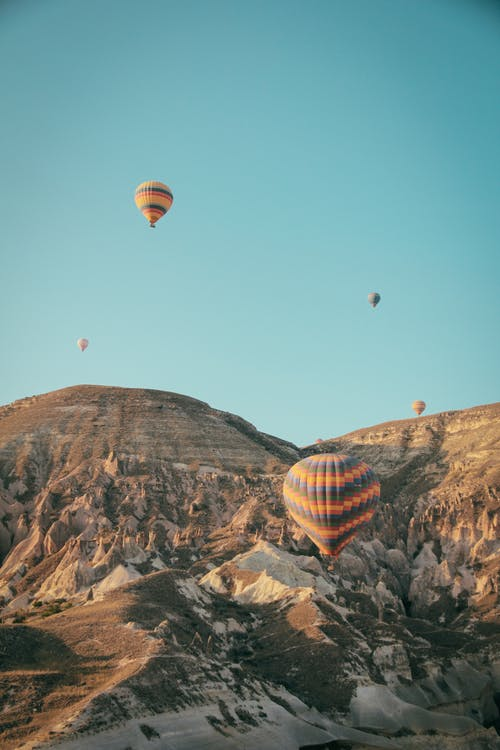
\includegraphics[width=0.5\columnwidth]{Chapters/Chapter1/Figures/Actors_SG}
\caption{Sample Image}
\label{Actors_SG}
\end{figure}


\section{LITERATURE REVIEW} % New Section Format
\subsection{Constituents of Advanced Metering Infrastructure} % New Sub-Section Format
Paragraph text goes here.

\subsubsection*{A. \textit{Advanced Metering Infrastructure}} % New Sub-Sub-Section Format
Advanced metering infrastructure (AMI) is an integrated system of smart energy meters (SEM), communication networks, and meter data management systems (MDMS) that enables bidirectional communication between utilities and consumers [\cite{park2010}]. 

\subsubsection*{B. \textit{Load Monitoring in AMI}}
Paragraph text goes here.

\section{OBJECTIVE AND SCOPE OF THE PRESENT RESEARCH WORK} % Objective and Scope Format
\noindent The objectives of the present research work are as follows:

\begin{enumerate}[itemsep=0.2cm,topsep=1pt,parsep=0pt,partopsep=0pt]
\item First Novel Point
\begin{itemize}[itemsep=0cm,topsep=2pt]
\item supportive statements;
\item benefits;
\end{itemize}
\item Second Novel Point
\begin{itemize}[itemsep=0cm,topsep=2pt]
\item supportive statements;
\item benefits;
\end{itemize}

\end{enumerate}

The scope of the present research work adopts a steady state modeling of household appliances from [\cite{arun2017}]. Replace existing sample paragraphs with your paragraphs.

\section{ORGANIZATION OF THESIS}
\noindent \textbf{Chapter 2:} This chapter deals with.

\noindent \textbf{Chapter 3:} In this chapter.